\chapter{Bouwplannen en weefsels van dieren}\label{ch:b1:body-plans-tissues}

Vier dieren op een laboratoriumtafel: een hydra van een centimeter, een
regenworm, een rivierkreeft, een kikker. Onder de verschillen in grootte en
levenswijze zijn zij gebouwd op een handvol gedeelde beslissingen --- of het
lichaam een voor- en een achterkant heeft, uit hoeveel cellagen het is gegroeid,
of er een holte rond de darm ligt, of het lichaam uit herhaalde segmenten
bestaat, waar het \omterm{def:b1:body-plans-tissues:segments}{skelet} zit --- en elk van hen is opgebouwd uit dezelfde vier
soorten \omterm{def:b1:body-plans-tissues:tissue}{weefsel}. Dit hoofdstuk zet de bouwplannen van dieren uiteen en de
\omterm{def:b1:body-plans-tissues:tissue}{weefsels} die ze opbouwen, en eindigt waar de vorige hoofdstukken ophielden: bij
de wand van een zoogdierdarm, gezien als \omterm{def:b1:body-plans-tissues:tissue}{weefsels} die tot een \omterm{def:b1:mammal-organization:organ}{orgaan} zijn
samengevoegd.

\section{Bouwplannen}

\begin{definition}[Symmetrie en cefalisatie]\label{def:b1:body-plans-tissues:symmetry}
Een dier heeft \emph{radiale symmetrie}\index{radiale symmetrie} wanneer zijn
lichaam rond een centrale as is geordend zonder links en rechts, zoals bij een
hydra of een kwal: het treedt zijn omgeving van alle kanten gelijk tegemoet, en
zit meestal vast of drijft mee. Het heeft \emph{bilaterale
symmetrie}\index{bilaterale symmetrie} wanneer één vlak het in spiegelbeeldige
helften verdeelt, met een voorzijde (anterieur) en een achterzijde (posterieur),
een rug (dorsaal) en een buik (ventraal): het plan van een dier dat zich met de
kop vooruit voortbeweegt, met de zintuigen en de zenuwcentra vooraan
geconcentreerd (\omterm{def:b1:mammal-organization:bodyplan}{cefalisatie}).
\end{definition}

\begin{definition}[Kiembladen, lichaamsholten]\label{def:b1:body-plans-tissues:layers}
Het embryo van een dier vormt twee of drie cellagen, de
\emph{kiembladen}\index{kiemblad}, waaruit alle \omterm{def:b1:body-plans-tissues:tissue}{weefsels} ontstaan: het
buitenste \emph{ectoderm}\index{ectoderm} (huid, zenuwstelsel), het
binnenste \emph{endoderm}\index{endoderm} (de bekleding van de darm en haar
uitstulpingen) en, bij alle dieren behalve de sponzen en de neteldieren, een
middelste \emph{mesoderm}\index{mesoderm} (spier, \omterm{def:b1:body-plans-tissues:segments}{skelet}, \omterm{def:b1:body-plans-tissues:connective}{bindweefsel}, bloed,
nieren, geslachtsklieren). Neteldieren zijn \emph{diploblastisch}, de rest
\emph{triploblastisch}. Bij triploblastische dieren kan het mesoderm de ruimte
tussen darm en lichaamswand opvullen (\emph{acoelomaat}: platwormen), of er een
holte tussen laten: een \emph{coeloom}\index{coeloom} wanneer die holte volledig
door mesoderm is bekleed (ringwormen, weekdieren, geleedpotigen,
stekelhuidigen, gewervelden). Het coeloom hangt de darm in een eigen
compartiment op, laat haar onafhankelijk van de lichaamswand bewegen, en geeft
zachtlijvige dieren een \omterm{def:b1:body-plans-tissues:segments}{hydrostatisch skelet}.
\end{definition}

\begin{omfigure}
\begin{tikzpicture}[font=\footnotesize, line cap=round]
  \node[font=\small, anchor=south] at (1.4,2.75) {acoelomaat (platworm)};
  \node[font=\small, anchor=south] at (6.6,2.75) {coelomaat (ringworm, gewervelde)};
  % acoelomate: body wall ectoderm, solid mesoderm, gut endoderm
  \draw[thick, fill=omDef!25] (1.4,1.3) ellipse (1.35 and 1.25);
  \fill[omProp!35] (1.4,1.3) ellipse (1.15 and 1.05);
  \draw[thick, fill=omExo!30] (1.4,1.3) ellipse (0.4 and 0.35);
  \node at (1.4,1.3) {darm};
  \node at (1.4,0.62) {mesoderm};
  % coelomate: body wall, coelom, gut with mesoderm layer
  \draw[thick, fill=omDef!25] (6.6,1.3) ellipse (1.35 and 1.25);
  \fill[omProp!35] (6.6,1.3) ellipse (1.15 and 1.05);
  \fill[white] (6.6,1.3) ellipse (0.95 and 0.85);
  \draw[thick, fill=omProp!35] (6.6,1.3) ellipse (0.55 and 0.5);
  \draw[thick, fill=omExo!30] (6.6,1.3) ellipse (0.4 and 0.35);
  \node at (6.6,1.3) {darm};
  \node at (6.6,0.62) {coeloom};
  % legend
  \fill[omDef!25] (8.9,2.2) rectangle +(0.35,0.25); \node[anchor=west] at (9.3,2.32) {ectoderm};
  \fill[omProp!35] (8.9,1.7) rectangle +(0.35,0.25); \node[anchor=west] at (9.3,1.82) {mesoderm};
  \fill[omExo!30] (8.9,1.2) rectangle +(0.35,0.25); \node[anchor=west] at (9.3,1.32) {endoderm};
  \draw (8.9,0.7) rectangle +(0.35,0.25); \node[anchor=west] at (9.3,0.82) {coeloom (holte)};
\end{tikzpicture}

{\small Dwarsdoorsneden van twee triploblastische bouwplannen. Bij de
acoelomaat vult het \omterm{def:b1:body-plans-tissues:layers}{mesoderm} de ruimte tussen lichaamswand en darm; bij de
coelomaat scheidt een met \omterm{def:b1:body-plans-tissues:layers}{mesoderm} beklede holte ze, zodat de darm vrij hangt
en de vloeistof in de holte als \omterm{def:b1:body-plans-tissues:segments}{skelet} kan dienen.}
\end{omfigure}

\begin{definition}[Protostomen en deuterostomen]\label{def:b1:body-plans-tissues:proto}
Bij de coelomate dieren verdeelt het lot van de eerste opening van de
embryonale darm twee grote lijnen: bij de \emph{protostomen}\index{protostoom}
(ringwormen, weekdieren, geleedpotigen) wordt zij de mond, ontstaat het \omterm{def:b1:body-plans-tissues:layers}{coeloom}
door splijting van het \omterm{def:b1:body-plans-tissues:layers}{mesoderm}, en verlopen de eerste eideligen spiraalvormig
met een vroeg vastgelegd lot; bij de
\emph{deuterostomen}\index{deuterostoom} (stekelhuidigen, gewervelden) wordt zij
de anus, ontstaat het \omterm{def:b1:body-plans-tissues:layers}{coeloom} door uitstulping van de darm, en blijft het lot
van de eerste cellen flexibel.
\end{definition}

\begin{definition}[Segmentatie, skeletten]\label{def:b1:body-plans-tissues:segments}
Een lichaam is \emph{gesegmenteerd}\index{segmentatie} wanneer het is opgebouwd
uit langs zijn as herhaalde eenheden (de ringen van een regenworm, de segmenten
van een rivierkreeft, de wervels en spierblokken van een vis), elk met een eigen
stel spieren, zenuwen en vaak aanhangsels. Segmenten kunnen gelijk zijn of tot
regio's gespecialiseerd (kop, borststuk, achterlijf). Het
\emph{skelet}\index{skelet} waartegen de spieren trekken is
\emph{hydrostatisch}\index{hydrostatisch skelet} (een vloeistof onder druk in
een \omterm{def:b1:body-plans-tissues:layers}{coeloom}, zoals bij de regenworm), een \emph{exoskelet}\index{exoskelet}
(een stijve \omterm{def:b1:flowering-plant-organization:tissues}{cuticula} buiten het lichaam, geleed, dat bij de groei wordt
vervangen, zoals bij geleedpotigen), of een \emph{endoskelet}\index{endoskelet}
(kraakbeen of bot binnen het lichaam, dat mee groeit, zoals bij gewervelden).
\end{definition}

\begin{omfigure}
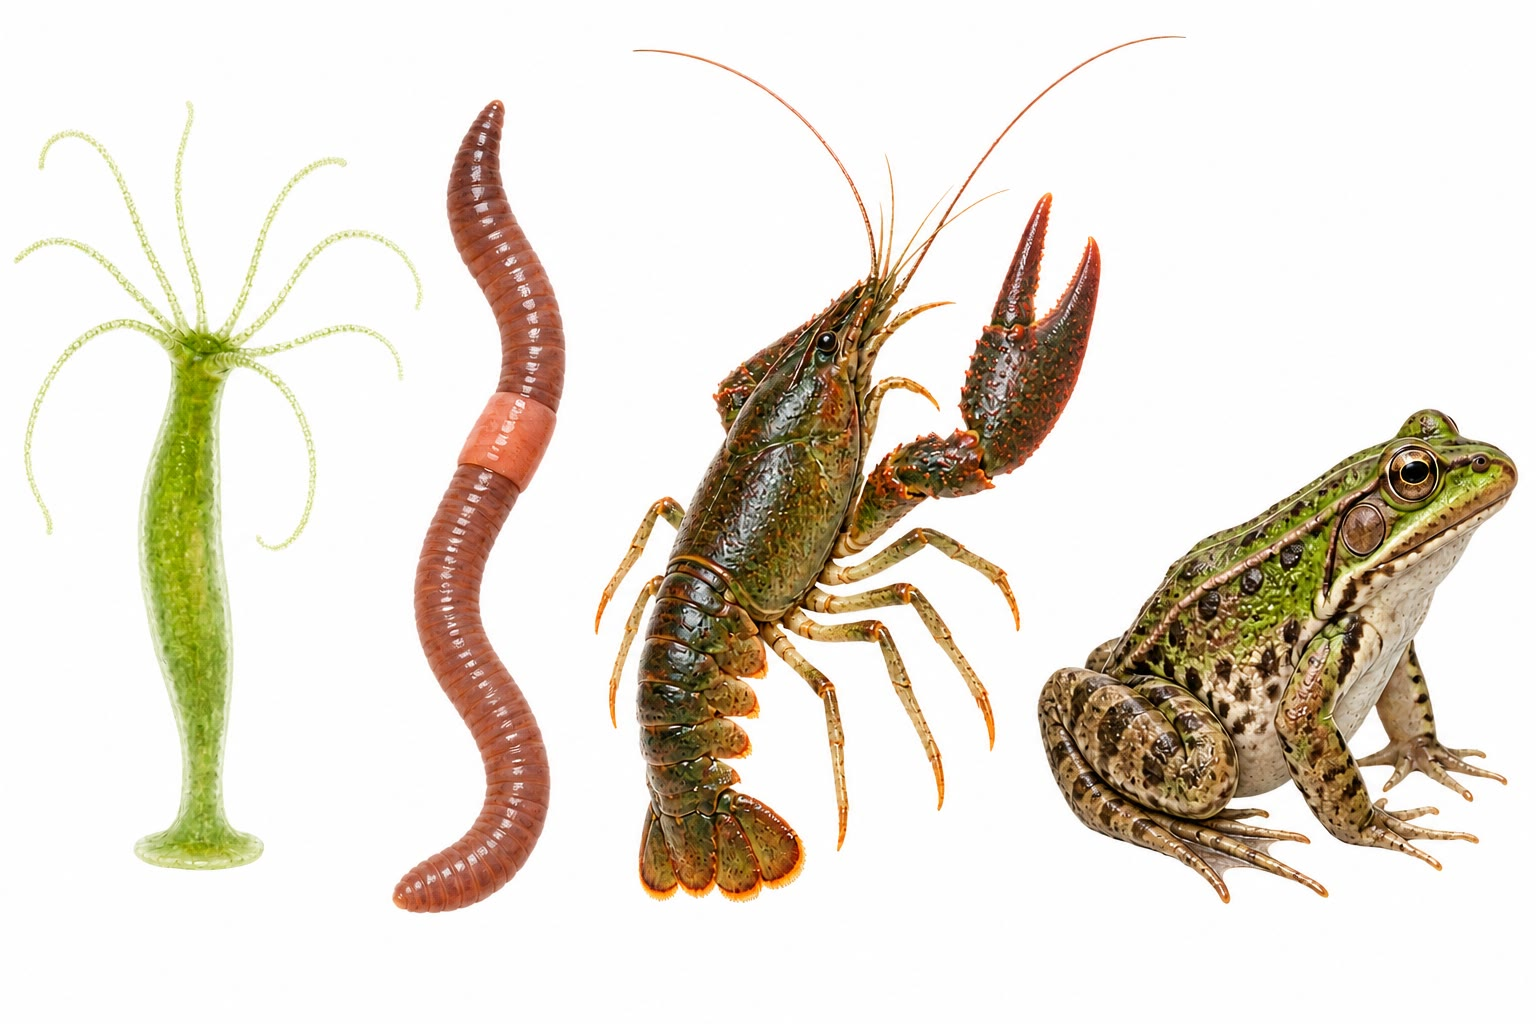
\includegraphics[width=0.78\linewidth]{images/book3/ai/b3-04-body-plans.jpg}

{\small Vier bouwplannen. Een hydra (radiaal, twee lagen, geen \omterm{def:b1:body-plans-tissues:layers}{coeloom}), een
regenworm (bilateraal, coelomaat, \omterm{def:b1:body-plans-tissues:segments}{gesegmenteerd}, \omterm{def:b1:body-plans-tissues:segments}{hydrostatisch skelet}), een
rivierkreeft (\omterm{def:b1:body-plans-tissues:segments}{gesegmenteerd} met gespecialiseerde regio's, geleed \omterm{def:b1:body-plans-tissues:segments}{exoskelet}) en
een kikker (\omterm{def:b1:body-plans-tissues:proto}{deuterostoom}, \omterm{def:b1:body-plans-tissues:segments}{endoskelet} van bot).}
\end{omfigure}

\begin{proposition}[Vier bouwplannen vergeleken]\label{prop:b1:body-plans-tissues:four}
\begin{center}
\small
\begin{tabular}{lllll}
\hline
 & hydra & regenworm & rivierkreeft & kikker \\
\hline
symmetrie & radiaal & bilateraal & bilateraal & bilateraal \\
kiembladen & 2 & 3 & 3 & 3 \\
\omterm{def:b1:body-plans-tissues:layers}{coeloom} & geen & ja & gereduceerd & ja \\
lijn & --- & \omterm{def:b1:body-plans-tissues:proto}{protostoom} & \omterm{def:b1:body-plans-tissues:proto}{protostoom} & \omterm{def:b1:body-plans-tissues:proto}{deuterostoom} \\
segmenten & nee & gelijk & gespecialiseerd & wervels, spierblokken \\
\omterm{def:b1:body-plans-tissues:segments}{skelet} & hydrostatisch & hydrostatisch & \omterm{def:b1:body-plans-tissues:segments}{exoskelet} & \omterm{def:b1:body-plans-tissues:segments}{endoskelet} \\
darm & één opening & mond tot anus & mond tot anus & mond tot anus \\
bloedsomloop & geen & gesloten & open & gesloten, hart \\
zenuwstelsel & net & buikstreng & buikstreng & rugstreng \\
\hline
\end{tabular}
\end{center}
De plannen zijn geen treden op een ladder: elk is een volledige en geslaagde
manier om een dier te zijn, en de rivierkreeft en de kikker zijn elkaars
tijdgenoten, niet elkaars voorouders.
\end{proposition}

\begin{example}[Een dier uit zijn plan lezen]\label{ex:b1:body-plans-tissues:reading}
Een dier met een kopeinde, een doorlopende darm, een lichaam van gelijkvormige
ringen en geen harde delen: een coelomate \omterm{def:b1:body-plans-tissues:proto}{protostoom} die zich met een
\omterm{def:b1:body-plans-tissues:segments}{hydrostatisch skelet} voortbeweegt, waarbij de coeloomvloeistof van elk segment
beurtelings door kringspieren en lengtespieren onder druk wordt gezet --- een
gravende regenworm. Een dier met een gelede \omterm{def:b1:flowering-plant-organization:tissues}{cuticula} en gespecialiseerde
segmenten: een geleedpotige, wiens groei door vervellingen moet gaan.
Bilateraal, met gesegmenteerde spierblokken rond een rugas van wervels: een
gewervelde, wiens \omterm{def:b1:body-plans-tissues:segments}{endoskelet} onafgebroken meegroeit.
\end{example}

\section{De vier weefseltypen}

\begin{definition}[Weefsel]\label{def:b1:body-plans-tissues:tissue}
Een \emph{weefsel}\index{weefsel} is een groep cellen van gelijke bouw en
herkomst, samen met het extracellulaire materiaal dat zij voortbrengen, zo
geordend dat zij een gemeenschappelijke functie vervullen. Dierlijke weefsels
vallen in vier typen uiteen: epitheel-, bind-, spier- en \omterm{def:b1:body-plans-tissues:nervous}{zenuwweefsel}. Elk
\omterm{def:b1:mammal-organization:organ}{orgaan} is een combinatie van ten minste twee ervan.
\end{definition}

\begin{definition}[Epitheelweefsel]\label{def:b1:body-plans-tissues:epithelium}
Een \emph{epitheel}\index{epitheel} is een laag dicht opeengepakte cellen die
een oppervlak bedekt of een holte bekleedt, rustend op een dunne laag
\omterm{def:b1:body-plans-tissues:connective}{extracellulaire matrix}, de \emph{basale lamina}\index{basale lamina}. Zijn
cellen zijn \emph{gepolariseerd}\index{celpolariteit}: de apicale zijde kijkt
naar de buitenwereld of naar het lumen, de basale zijde naar de lamina, en de
twee dragen verschillende eiwitten. Zij worden verbonden door
\emph{celverbindingen}\index{celverbinding}: \emph{tight junctions} vlak bij de
top, die de ruimte tussen de cellen afdichten zodat niets de laag passeert
behalve door de cellen heen; \emph{adherens junctions} en
\emph{desmosomen}, die de cellen mechanisch vastzetten; \emph{gap
junctions}, kanalen die ionen en kleine moleculen van cel naar cel laten gaan.
Epithelia worden ingedeeld naar het aantal lagen (enkelvoudig, meerlagig) en de
vorm van de cellen (plaveisel, kubisch, cilindrisch), en omvatten de klieren,
epitheelcellen die in afscheiding zijn gespecialiseerd. Zij bedekken,
beschermen, nemen op en scheiden af.
\end{definition}

\begin{omfigure}
\begin{tikzpicture}[font=\footnotesize, line cap=round]
  % three columnar cells
  \foreach \x in {0,1.6,3.2} {
    \draw[thick, fill=omDef!10] (\x,0) rectangle (\x+1.5,3.2);
    \fill[omDef!60] (\x+0.75,0.9) ellipse (0.32 and 0.42);
    % microvilli
    \foreach \m in {0.15,0.35,0.55,0.75,0.95,1.15,1.35} \draw[omDef!70!black, thick] (\x+\m,3.2) -- (\x+\m,3.5);
  }
  % junctions between cell 1-2 and 2-3
  \foreach \x in {1.55,3.15} {
    \draw[very thick, omThm] (\x-0.05,2.9) -- (\x+0.1,2.9);
    \draw[very thick, omProp] (\x-0.05,2.5) -- (\x+0.1,2.5);
    \draw[very thick, omProp] (\x-0.05,1.9) -- (\x+0.1,1.9);
    \draw[very thick, omExo] (\x-0.05,1.2) -- (\x+0.1,1.2);
  }
  % basal lamina
  \draw[very thick, gray!70] (-0.2,-0.05) -- (4.9,-0.05);
  \fill[pattern=north east lines, pattern color=gray!50] (-0.2,-0.6) rectangle (4.9,-0.1);
  % labels
  \node[anchor=south] at (2.4,3.55) {apicale zijde: microvilli, naar het lumen};
  \node[anchor=west, omThm] at (5.1,2.9) {tight junction: dicht de spleet af};
  \node[anchor=west, omProp] at (5.1,2.5) {adherens junction: actinegordel};
  \node[anchor=west, omProp] at (5.1,1.9) {desmosoom: mechanische klinknagel};
  \node[anchor=west, omExo] at (5.1,1.2) {gap junction: kanaal van cel tot cel};
  \node[anchor=west, gray!80!black] at (5.1,-0.05) {basale lamina};
  \node[anchor=west, gray!80!black] at (5.1,-0.45) {bindweefsel eronder};
  \node[anchor=east] at (-0.3,0.9) {celkern};
\end{tikzpicture}

{\small Een enkelvoudig cilindrisch \omterm{def:b1:body-plans-tissues:epithelium}{epitheel}, zoals in de darm. Elke cel heeft
een apicale zijde met microvilli en een basale zijde op de \omterm{def:b1:body-plans-tissues:epithelium}{basale lamina};
buren zijn afgedicht door tight junctions, vastgezet door adherens junctions en
desmosomen, en verbonden door gap junctions.}
\end{omfigure}

\begin{definition}[Bindweefsel]\label{def:b1:body-plans-tissues:connective}
\emph{Bindweefsel}\index{bindweefsel} bestaat uit verspreide cellen in een
overvloedige \emph{extracellulaire matrix}\index{extracellulaire matrix} die
zij afscheiden: eiwitvezels --- \emph{collageen}\index{collageen}
(treksterkte; een kwart van alle eiwit in een zoogdier),
\emph{elastine}\index{elastine} (veerkracht) --- ingebed in een gehydrateerde
\emph{grondsubstantie} van polysachariden. De verhoudingen bepalen de typen:
los bindweefsel onder epithelia en rond \omterm{def:b1:mammal-organization:organ}{organen} (fibroblasten, weinig vezels,
veel grondsubstantie); vast bindweefsel van pezen en gewrichtsbanden (evenwijdig
collageen); vetweefsel (vetopslaande cellen); kraakbeen (een stevige gel van
collageen en polysachariden, zonder bloedvaten); bot (collageen gemineraliseerd met
calciumfosfaat, levende cellen in holten, bloedvaten); en bloed, waarvan de matrix
het \omterm{def:b1:mammal-organization:compartments}{plasma} is. Het bindt, steunt, slaat op, vervoert en verdedigt.
\end{definition}

\begin{definition}[Spierweefsel]\label{def:b1:body-plans-tissues:muscle}
\emph{Spierweefsel}\index{spierweefsel} bestaat uit langgerekte cellen
volgepakt met samentrekkende eiwitfilamenten (actine en myosine). Er zijn drie
typen: \emph{skeletspier}, met lange meerkernige vezels die dwarsstreping
vertonen, aan het \omterm{def:b1:body-plans-tissues:segments}{skelet} vastgehecht en willekeurig aanstuurbaar;
\emph{hartspier}, met vertakte dwarsgestreepte cellen die kop aan staart
verbonden zijn door verbindingen die de slag van cel naar cel doorgeven, en die
op een eigen ritme samentrekt; \emph{gladde spier}, met spoelvormige
ongestreepte cellen in de wanden van holle \omterm{def:b1:mammal-organization:organ}{organen} (darm, bloedvaten, baarmoeder),
die traag en onwillekeurig samentrekt. Het mechanisme van de samentrekking komt
aan bod in het deel van jaar 2.
\end{definition}

\begin{definition}[Zenuwweefsel]\label{def:b1:body-plans-tissues:nervous}
\emph{Zenuwweefsel}\index{zenuwweefsel} bestaat uit
\emph{neuronen}\index{neuron}, cellen met een lichaam en lange uitlopers
(dendrieten die signalen ontvangen, een axon dat ze wegvoert) die elektrische
signalen geleiden en ze bij synapsen aan andere cellen doorgeven, en uit
\emph{gliacellen}\index{gliacel}, die enkele keren talrijker zijn en de neuronen
ondersteunen, isoleren en voeden. Het neemt waar, integreert en stuurt aan.
\end{definition}

\begin{omfigure}
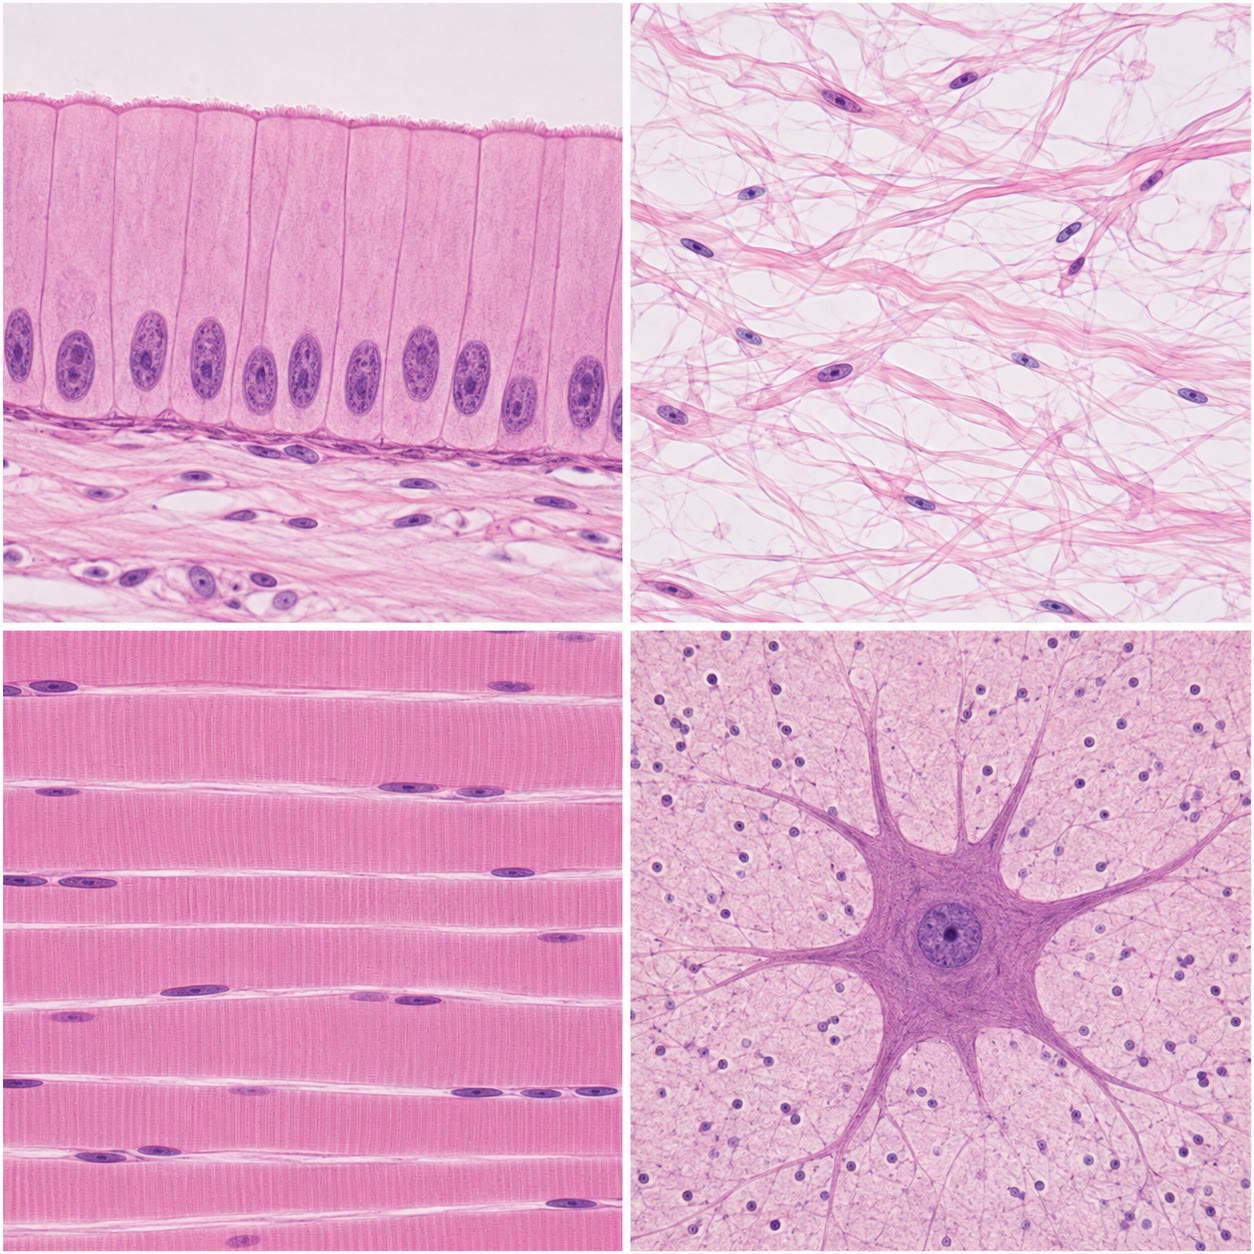
\includegraphics[width=0.6\linewidth]{images/book3/ai/b3-04-tissues.jpg}

{\small De vier weefseltypen onder de microscoop. Linksboven: enkelvoudig
cilindrisch \omterm{def:b1:body-plans-tissues:epithelium}{epitheel}, één rij hoge cellen. Rechtsboven: los \omterm{def:b1:body-plans-tissues:connective}{bindweefsel},
verspreide cellen tussen golvende collageenvezels. Linksonder: dwarsgestreepte
skeletspiervezels met de kernen aan hun rand. Rechtsonder: een \omterm{def:b1:body-plans-tissues:nervous}{neuron} tussen
\omterm{def:b1:body-plans-tissues:nervous}{gliacellen}.}
\end{omfigure}

\begin{example}[Waar de weefsels vandaan komen]\label{ex:b1:body-plans-tissues:origin}
Epithelia komen uit alle drie de kiembladen voort (de huid uit \omterm{def:b1:body-plans-tissues:layers}{ectoderm}, de
darmbekleding uit \omterm{def:b1:body-plans-tissues:layers}{endoderm}, de bekleding van de bloedvaten en van het \omterm{def:b1:body-plans-tissues:layers}{coeloom} uit
\omterm{def:b1:body-plans-tissues:layers}{mesoderm}); \omterm{def:b1:body-plans-tissues:connective}{bindweefsel}, spier en bloed uit \omterm{def:b1:body-plans-tissues:layers}{mesoderm}; \omterm{def:b1:body-plans-tissues:nervous}{zenuwweefsel} uit \omterm{def:b1:body-plans-tissues:layers}{ectoderm}.
De huid van de kikker is een ectodermaal \omterm{def:b1:body-plans-tissues:epithelium}{epitheel} op mesodermaal \omterm{def:b1:body-plans-tissues:connective}{bindweefsel};
zijn darm een endodermaal \omterm{def:b1:body-plans-tissues:epithelium}{epitheel} omhuld door mesodermale spier; zijn hersenen
naar binnen gevouwen \omterm{def:b1:body-plans-tissues:layers}{ectoderm}.
\end{example}

\section{Van weefsels naar een orgaan: de darmwand}

\begin{proposition}[De vier lagen van de darmwand]\label{prop:b1:body-plans-tissues:gutwall}
\index{darmwand}
Van het lumen naar buiten is de wand van de spijsverteringsbuis van een
gewervelde opgebouwd uit vier concentrische lagen, elk een combinatie van
\omterm{def:b1:body-plans-tissues:tissue}{weefsels}: de \emph{mucosa} (een \omterm{def:b1:body-plans-tissues:epithelium}{epitheel} --- opnemend en afscheidend --- op los
\omterm{def:b1:body-plans-tissues:connective}{bindweefsel} met bloedvaten en lymfevaten, met daaronder een dunne laag gladde spier);
de \emph{submucosa} (vast \omterm{def:b1:body-plans-tissues:connective}{bindweefsel} met grotere bloedvaten en een zenuwnetwerk); de
\emph{muscularis} (twee lagen gladde spier, binnen circulair en buiten
longitudinaal, met een zenuwnetwerk ertussen, die de mengende en voortstuwende
bewegingen voortbrengen); en de \emph{serosa} (een dunne bindweefsellaag bedekt
door het \omterm{def:b1:body-plans-tissues:epithelium}{epitheel} van het \omterm{def:b1:body-plans-tissues:layers}{coeloom}). Dezelfde vier lagen lopen van slokdarm tot
endeldarm; wat verandert is de mucosa --- in de dunne darm tot darmvlokken
geplooid, in de maag klierrijk.
\end{proposition}

\begin{omfigure}
\begin{tikzpicture}
  \node[anchor=south west, inner sep=0] (img) at (0,0)
    {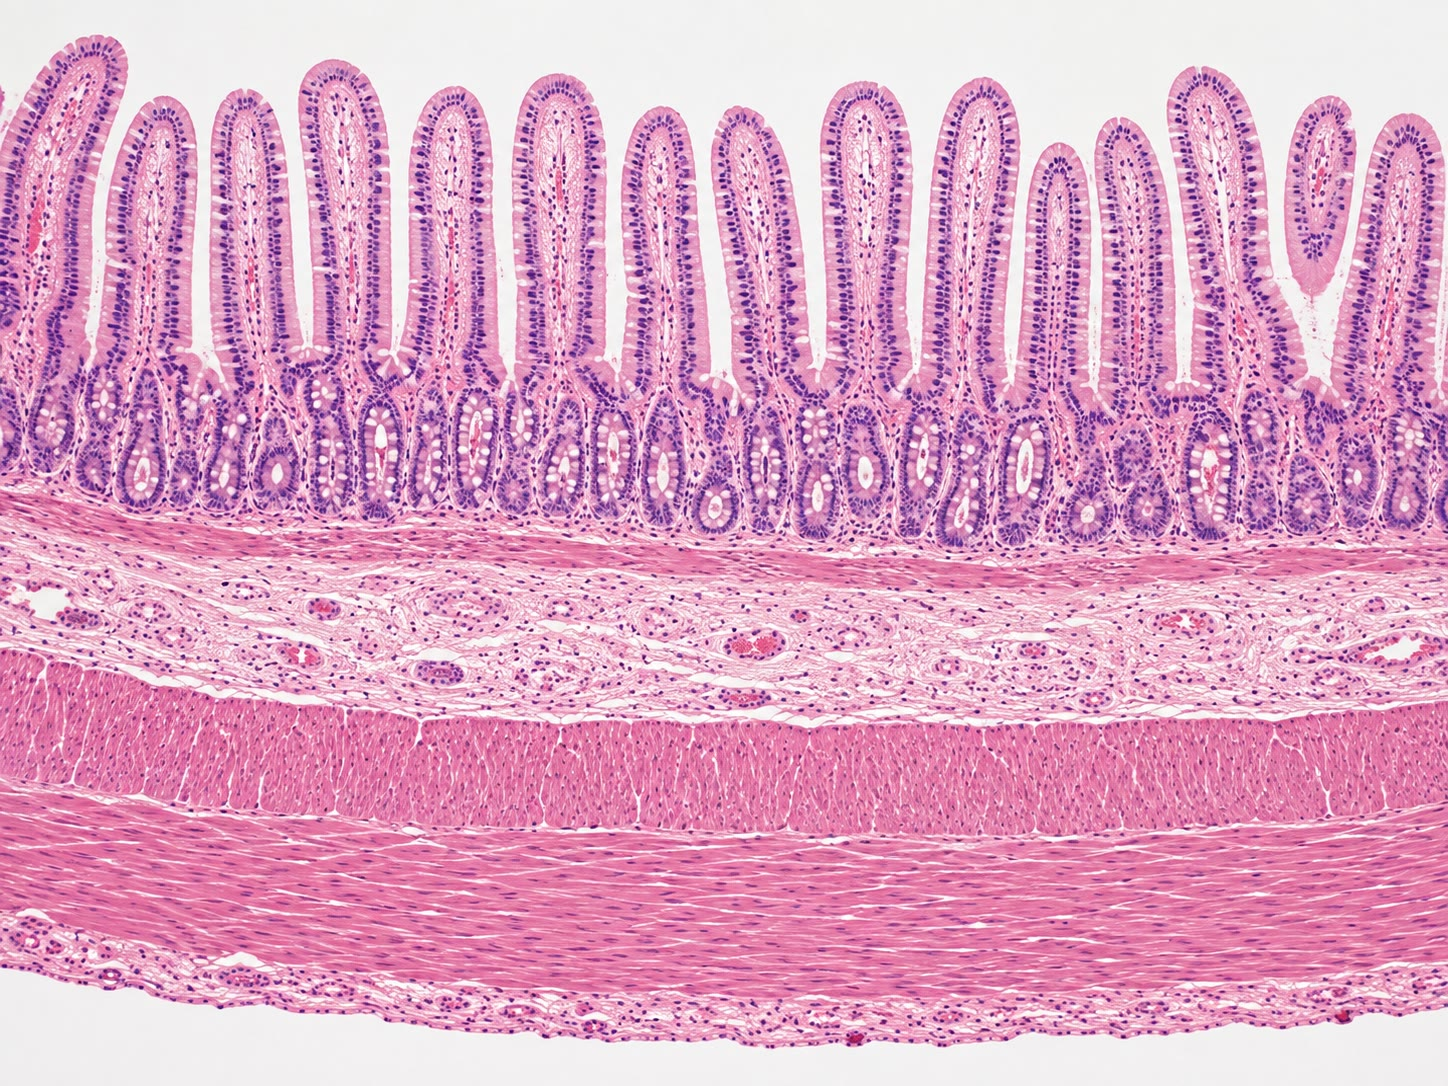
\includegraphics[width=0.53\linewidth]{images/book3/ai/fig-gut-wall-histology.jpg}};
  \begin{scope}[x={(img.south east)}, y={(img.north west)},
      every node/.style={font=\small}]
    \draw[omDef, thick] (0.50,0.985) -- (0.50,1.08) node[above] {lumen};
    \draw[omDef, thick] (0.30,0.82) -- (-0.03,0.86) node[left, align=right] {darmvlok: epitheel\\ op bindweefsel};
    \draw[omDef, thick] (0.40,0.58) -- (-0.03,0.56) node[left] {klieren (crypten)};
    \draw[omDef, thick] (0.70,0.505) -- (1.03,0.56) node[right] {muscularis mucosae};
    \draw[omDef, thick] (0.70,0.42) -- (1.03,0.42) node[right] {submucosa};
    \draw[omDef, thick] (0.70,0.24) -- (1.03,0.26) node[right, align=left] {muscularis:\\ circulair,\\ longitudinaal};
    \draw[omDef, thick] (0.70,0.06) -- (1.03,0.06) node[right] {serosa};
  \end{scope}
\end{tikzpicture}

{\small Dwarsdoorsnede van de wand van de dunne darm. Darmvlokken van de mucosa
steken het lumen in; daaronder de klieren, een dunne spierlaag, de submucosa, de
twee lagen van de muscularis en de serosa. Vier lagen, vier weefseltypen, één
\omterm{def:b1:mammal-organization:organ}{orgaan}.}
\end{omfigure}

\begin{method}[Een histologisch preparaat lezen]\label{met:b1:body-plans-tissues:histology}
\begin{enumerate}
  \item Zoek het vrije oppervlak of het lumen: het \omterm{def:b1:body-plans-tissues:epithelium}{epitheel} dat het
        bekleedt is de eerste laag. Tel het aantal rijen kernen
        (enkelvoudig of meerlagig) en let op de vorm van de cellen.
  \item Zoek onder het \omterm{def:b1:body-plans-tissues:epithelium}{epitheel} de bleke, vezelige zone met verspreide
        kernen en bloedvaten: \omterm{def:b1:body-plans-tissues:connective}{bindweefsel}.
  \item Spier verschijnt als dichte bundels langgerekte cellen:
        dwarsgestreept met randstandige kernen (\omterm{def:b1:body-plans-tissues:segments}{skelet}), dwarsgestreept en
        vertakt (hart), ongestreept met een centrale kern (glad). Let op
        de richting van de vezels ten opzichte van het preparaat.
  \item \omterm{def:b1:body-plans-tissues:nervous}{Zenuwweefsel} in een orgaanwand verschijnt als groepjes grote
        bleke neuronlichamen tussen de spierlagen.
  \item Benoem het \omterm{def:b1:mammal-organization:organ}{orgaan} aan de hand van de opeenvolging van de lagen en
        de bijzonderheden van de mucosa (darmvlokken, klieren, keratine).
\end{enumerate}
\end{method}

\begin{example}[De darmvlok als uitwisselingsoppervlak]\label{ex:b1:body-plans-tissues:villus}
Een darmvlok van de menselijke dunne darm is een vinger van \qty{0.6}{mm} hoog
en \qty{0.15}{mm} breed, bedekt door één laag cilindrische cellen waarvan de
apicale zijden elk zo'n \qty{1500}{} microvilli dragen. Darmvlokken
vermenigvuldigen het oppervlak van de buis ongeveer zevenvoudig en microvilli
nog eens twintigvoudig: de \qty{0.6}{m^2} van een gladde buis wordt tientallen
vierkante meters opnemend \omterm{def:b1:body-plans-tissues:epithelium}{epitheel} van één cel dik, waarbij elke cel op enkele
micrometers van een haarvat en een lymfevat in de bindweefselkern van haar
darmvlok ligt (\cref{ch:b1:digestion-absorption}). Het \omterm{def:b1:body-plans-tissues:epithelium}{epitheel} wordt vanuit de
klieren aan zijn voet elke vier dagen vernieuwd: de laag, haar verbindingen en
haar polariteit worden voortdurend opnieuw opgebouwd.
\end{example}

\begin{remark}[De weefsels van de twee modelorganismen]\label{rem:b1:body-plans-tissues:plants}
De drie weefselstelsels van de plant uit
\cref{ch:b1:flowering-plant-organization} hebben hier geen exacte tegenhangers.
Haar epidermis is naar functie een \omterm{def:b1:body-plans-tissues:epithelium}{epitheel}, maar haar cellen worden door wanden
bijeengehouden en niet door verbindingen; haar \omterm{def:b1:flowering-plant-organization:tissues}{grondweefsel} is tegelijk opslag,
steun en fotosynthetisch; zij heeft spier noch zenuw. De vier \omterm{def:b1:body-plans-tissues:tissue}{weefsels} van het
dier zijn het gereedschap van een lichaam dat beweegt en waarneemt; de drie van
de plant dat van een lichaam dat groeit.
\end{remark}

\section{Opgaven}

\begin{exercise}[$\star$]\label{exo:b1:body-plans-tissues:1}
Definieer radiale en \omterm{def:b1:body-plans-tissues:symmetry}{bilaterale symmetrie} en geef van elk een dier. Welke gaat
samen met \omterm{def:b1:mammal-organization:bodyplan}{cefalisatie}, en waarom?
\end{exercise}

\begin{exercise}[$\star$]\label{exo:b1:body-plans-tissues:2}
Noem de drie kiembladen en van elk één afgeleid \omterm{def:b1:body-plans-tissues:tissue}{weefsel}.
\end{exercise}

\begin{exercise}[$\star$]\label{exo:b1:body-plans-tissues:3}
Noem de vier weefseltypen met hun kenmerkende eigenschap en van elk één functie.
\end{exercise}

\begin{exercise}[$\star$]\label{exo:b1:body-plans-tissues:4}
Noem aan de hand van de epitheelfiguur de vier verbindingen van de top tot de
basis en de taak van elk.
\end{exercise}

\begin{exercise}[$\star\star$]\label{exo:b1:body-plans-tissues:5}
Een dier heeft drie kiembladen, een met \omterm{def:b1:body-plans-tissues:layers}{mesoderm} beklede lichaamsholte, een
doorlopende darm, gelijkvormige segmenten en geen harde delen. Geef zijn
plankenmerken een voor een en noem een groep die erbij past.
\end{exercise}

\begin{exercise}[$\star\star$]\label{exo:b1:body-plans-tissues:6}
Leg uit hoe een regenworm zich voortbeweegt door zijn \omterm{def:b1:body-plans-tissues:layers}{coeloom} als \omterm{def:b1:body-plans-tissues:segments}{skelet} te
gebruiken, met de twee spierlagen van elk segment.
\end{exercise}

\begin{exercise}[$\star\star$]\label{exo:b1:body-plans-tissues:7}
Vergelijk het \omterm{def:b1:body-plans-tissues:segments}{exoskelet} van de rivierkreeft en het \omterm{def:b1:body-plans-tissues:segments}{endoskelet} van de kikker:
groei, bescherming, aanhechting van de spieren, en de grens aan de grootte die
elk oplegt.
\end{exercise}

\begin{exercise}[$\star\star$]\label{exo:b1:body-plans-tissues:8}
Waarom heeft een \omterm{def:b1:body-plans-tissues:epithelium}{epitheel} tight junctions nodig om een \omterm{prop:b1:organism-environment:surfaces}{uitwisselingsoppervlak}
onder controle van het \omterm{def:b1:organism-environment:organism}{organisme} te zijn? Wat zou er zonder die verbindingen met
de opname in de darm gebeuren?
\end{exercise}

\begin{exercise}[$\star\star$]\label{exo:b1:body-plans-tissues:9}
Een preparaat toont, van een lumen naar buiten: een enkelvoudig cilindrisch
\omterm{def:b1:body-plans-tissues:epithelium}{epitheel} met darmvlokken, los \omterm{def:b1:body-plans-tissues:connective}{bindweefsel}, een dunne spierlaag, vast \omterm{def:b1:body-plans-tissues:connective}{bindweefsel},
twee dikke spierlagen, een dunne buitenlaag. Benoem het \omterm{def:b1:mammal-organization:organ}{orgaan} en elke laag.
\end{exercise}

\begin{exercise}[$\star\star\star$]\label{exo:b1:body-plans-tissues:10}
Kraakbeen heeft geen bloedvaten en bot vele. Breng dat in verband met de manier
waarop elk wordt gevoed, hoe snel elk geneest, en waar elk in het lichaam wordt
gebruikt.
\end{exercise}

\begin{exercise}[$\star\star\star$]\label{exo:b1:body-plans-tissues:11}
Een geneesmiddel blokkeert de vorming van tight junctions in het darmepitheel.
Voorspel de gevolgen voor de opname, voor de samenstelling van het \omterm{def:b1:organism-environment:milieu}{intern milieu}
en voor infectie, aan de hand van de eigenschappen van epithelia.
\end{exercise}

\begin{exercise}[$\star\star\star$]\label{exo:b1:body-plans-tissues:12}
``Een \omterm{def:b1:mammal-organization:bodyplan}{bouwplan} is een stel beperkingen, geen ontwerp.'' Bespreek dat in een
alinea aan de hand van het vervellen van geleedpotigen, de grootte van insecten,
de segmenten van gewervelden, en de betekenis van de tabel in dit hoofdstuk.
\end{exercise}

\section{Vraagstuk: de wand van de dunne darm}

\begin{problem}[{Weekendvraagstuk --- een histologische reeks van de menselijke
dunne darm, gelezen van de buis tot aan de microvillus: lagen, darmvlokken,
cellen, verbindingen en vernieuwing, eindigend op het opnemende oppervlak van
één darmvlok}]
\label{pb:b1:body-plans-tissues:1}
De menselijke dunne darm is een buis van \qty{6}{m} lang met een inwendige
diameter van \qty{3}{cm}. Kringplooien van de wand verdrievoudigen het oppervlak
van de gladde buis. De mucosa draagt \qty{25}{} darmvlokken per vierkante
millimeter geplooid oppervlak, elk een cilinder van \qty{0.6}{mm} hoog en
\qty{0.15}{mm} in doorsnede. De darmvlokken zijn bedekt met cilindrische cellen
waarvan de apicale zijde een vierkant met zijde \qty{5}{\micro m} is; elke
apicale zijde draagt \qty{1500}{} microvilli, cilinders van \qty{1}{\micro m}
lang en \qty{0.1}{\micro m} in doorsnede. Het \omterm{def:b1:body-plans-tissues:epithelium}{epitheel} wordt elke \qty{4}{}
dagen vernieuwd.

\medskip
\noindent\textbf{Deel I --- De lagen.}
Een dwarsdoorsnede wordt onder de microscoop bekeken.
\begin{enumerate}
  \item Noem de vier lagen van de wand van het lumen naar buiten en de
        weefseltypen in elke laag.
  \item Het preparaat toont darmvlokken. Van welk deel van de
        spijsverteringsbuis is het? Wat zou een preparaat van de maag in
        plaats daarvan tonen?
  \item Tussen de twee spierlagen van de muscularis liggen groepjes grote
        bleke cellen. Wat zijn dat, en wat sturen zij aan?
  \item Leg uit waarom de twee spierlagen loodrecht op elkaar lopen.
\end{enumerate}

\medskip
\noindent\textbf{Deel II --- Oppervlakken.}
\begin{enumerate}[resume]
  \item Bereken het inwendige oppervlak van de gladde buis.
  \item Bereken het oppervlak na de kringplooien.
  \item Bereken het zijoppervlak van één darmvlok (cilinder, zonder de
        top).
  \item Bereken het darmvlokoppervlak per vierkante millimeter geplooide
        mucosa en de factor waarmee de darmvlokken het oppervlak
        vermenigvuldigen.
  \item Bereken het oppervlak na de darmvlokken.
  \item Bereken het zijoppervlak van één microvillus en van de
        \qty{1500}{} op één cel.
  \item Bereken de factor waarmee de microvilli het apicale oppervlak van
        een cel vermenigvuldigen.
  \item Bereken het totale opnemende oppervlak van de dunne darm.
\end{enumerate}

\medskip
\noindent\textbf{Deel III --- Cellen.}
\begin{enumerate}[resume]
  \item Bereken het aantal epitheelcellen dat één darmvlok bedekt.
  \item Bereken het aantal darmvlokken in de dunne darm en het aantal
        epitheelcellen dat ze bedekt.
  \item Het \omterm{def:b1:body-plans-tissues:epithelium}{epitheel} wordt elke \qty{4}{} dagen vernieuwd. Hoeveel cellen
        worden er per dag en per seconde in het lumen afgestoten?
  \item Waar worden de vervangende cellen gevormd, en wat zegt dat over de
        plaats van de delende cellen ten opzichte van de opnemende?
  \item Een epitheelcel is \qty{25}{\micro m} hoog. Bereken het volume van
        het \omterm{def:b1:body-plans-tissues:epithelium}{epitheel} in de dunne darm en de massa ervan (dichtheid
        \qty{1.05}{g/cm^3}).
\end{enumerate}

\medskip
\noindent\textbf{Deel IV --- Verbindingen, matrix en de darmvlok.}
\begin{enumerate}[resume]
  \item Elke cel is met een tight junction rondom haar top aan haar buren
        afgedicht. Bereken de lengte tight junction per cel en de totale
        lengte in de dunne darm.
  \item Leg uit waarom een stof in het lumen het bloed alleen kan bereiken
        door twee celmembranen te passeren.
  \item De kern van de darmvlok is los \omterm{def:b1:body-plans-tissues:connective}{bindweefsel} met een haarvatennet en
        een centraal lymfevat. Noem de twee typen extracellulaire vezel
        die zij bevat en de cel die ze afscheidt.
  \item Noem het \omterm{def:b1:body-plans-tissues:layers}{kiemblad} waaruit het \omterm{def:b1:body-plans-tissues:epithelium}{epitheel} en waaruit de kern
        voortkomen.
  \item De darmvlok bevat ook een streng gladde spier die haar ritmisch
        laat verkorten. Stel een functie daarvan voor.
  \item Een ziekte vlakt de darmvlokken af (het oppervlak keert terug naar
        dat van de geplooide buis). Met welke factor daalt het opnemende
        oppervlak, en wat zijn de gevolgen?
  \item Bereken het opnemende oppervlak van één darmvlok met haar
        microvilli, in vierkante millimeters.
  \item Geef het resultaat: het opnemende oppervlak van één darmvlok, en
        het aantal darmvlokken in de dunne darm.
\end{enumerate}
\end{problem}
